\section{Quantitative Analysis}

\subsection{Cluster Counting}
Table 5.1 below shows the frequency count of each cluster per symphony. Each time a point is found in a cluster, the frequency count of the corresponding label is incremented. Table 5.2 shows the percentage of the same frequency distribution table of clusters per symphony. Cluster label A has the highest number of frequency with a total of 86983, followed by B with 65867, E with 65355, D with 60726, and lastly, C with 51845. These cluster counts can be used to help verify the similarity of symphonies by, for example, checking the results from the metrics done later on and seeing whether their cluster counts are truly similar.

\begin{longtable}{|l|l|l|l|l|l|l|}
\caption{Frequency Cluster Count}
\label{my-label}\\
\hline
Row Labels & A & B & C & D & E & Grand Total \\ \hline
\endfirsthead
\endhead
%
P1C1S1 & 383 & 43 & 6 & 152 & 1 & 585 \\ \hline
P1C1S2 & 116 & 1609 & 2 & 16 & 710 & 2453 \\ \hline
P1C1S3 & 4 & 3 &  & 1 & 795 & 803 \\ \hline
P1C1S4 & 2 & 243 &  &  &  & 245 \\ \hline
P1C1S5 & 1 & 352 &  & 3 & 2 & 358 \\ \hline
P1C2S1 & 223 & 14 &  &  & 153 & 390 \\ \hline
P1C2S2 & 4 & 841 & 3 & 31 & 1 & 880 \\ \hline
P1C2S3 & 106 & 100 &  &  & 431 & 637 \\ \hline
P1C2S4 & 479 & 18 & 5 & 5 & 154 & 661 \\ \hline
P1C2S5 & 180 & 415 & 48 & 291 & 339 & 1273 \\ \hline
P1C3S1 & 1 & 41 &  &  & 596 & 638 \\ \hline
P1C3S2 & 450 & 73 & 5 & 32 & 71 & 631 \\ \hline
P1C3S3 &  & 90 &  & 1 & 227 & 318 \\ \hline
P1C3S4 & 2 & 10 &  & 387 &  & 399 \\ \hline
P1C3S5 & 276 & 2 &  & 1 & 23 & 302 \\ \hline
P1C4S1 & 58 & 99 & 20 & 82 & 22 & 281 \\ \hline
P1C4S2 & 83 & 109 &  & 2 & 783 & 977 \\ \hline
P1C4S3 & 297 & 286 & 83 & 408 & 57 & 1131 \\ \hline
P1C4S4 & 104 & 78 &  & 4 & 1344 & 1530 \\ \hline
P1C4S5 & 134 & 690 & 72 & 253 & 44 & 1193 \\ \hline
P1C5S1 & 33 & 952 & 2 & 1 & 24 & 1012 \\ \hline
P1C5S2 & 2 & 241 &  & 5 & 87 & 335 \\ \hline
P1C5S3 & 12 & 338 &  & 1 & 111 & 462 \\ \hline
P1C5S4 & 7 & 70 &  &  & 251 & 328 \\ \hline
P1C5S5 & 268 & 13 &  & 2 & 133 & 416 \\ \hline
P2C1S1 & 1369 & 643 & 228 & 414 & 121 & 2775 \\ \hline
P2C1S2 & 1055 & 827 & 77 & 398 & 180 & 2537 \\ \hline
P2C1S3 & 988 & 686 & 107 & 806 & 143 & 2730 \\ \hline
P2C1S4 & 1808 & 534 & 22 & 217 & 425 & 3006 \\ \hline
P2C1S5 & 478 & 148 & 18 & 90 & 232 & 966 \\ \hline
P2C2S1 & 86 & 91 & 40 & 40 & 191 & 448 \\ \hline
P2C2S2 & 180 & 258 & 60 & 270 & 110 & 878 \\ \hline
P2C2S3 & 336 & 1059 & 104 & 180 & 373 & 2052 \\ \hline
P2C2S4 & 353 & 287 & 39 & 32 & 454 & 1165 \\ \hline
P2C2S5 & 545 & 709 & 34 & 121 & 667 & 2076 \\ \hline
P2C3S1 & 279 & 369 & 12 & 22 & 249 & 931 \\ \hline
P2C3S2 & 72 & 206 & 2 & 8 & 804 & 1092 \\ \hline
P2C3S3 & 259 & 133 & 1 & 1 & 1218 & 1612 \\ \hline
P2C3S4 & 623 & 192 & 1 & 4 & 864 & 1684 \\ \hline
P2C3S5 & 504 & 123 & 6 & 81 & 599 & 1313 \\ \hline
P2C4S1 & 1396 & 330 & 16 & 44 & 1164 & 2950 \\ \hline
P2C4S2 & 764 & 612 & 421 & 265 & 845 & 2907 \\ \hline
P2C4S3 & 1082 & 293 & 71 & 162 & 913 & 2521 \\ \hline
P2C4S4 & 881 & 208 & 30 & 11 & 2112 & 3242 \\ \hline
P2C4S5 & 1091 & 546 & 492 & 271 & 771 & 3171 \\ \hline
P2C5S1 & 694 & 521 & 232 & 703 & 1446 & 3596 \\ \hline
P2C5S2 & 700 & 653 & 476 & 1144 & 80 & 3053 \\ \hline
P2C5S3 & 1375 & 373 & 539 & 792 & 281 & 3360 \\ \hline
P2C5S4 & 1145 & 1119 & 629 & 1408 & 26 & 4327 \\ \hline
P2C5S5 & 472 & 381 & 129 & 301 & 339 & 1622 \\ \hline
P3C1S1 & 514 & 411 & 87 & 296 & 46 & 1354 \\ \hline
P3C1S2 & 246 & 103 & 14 & 84 & 28 & 475 \\ \hline
P3C1S3 & 1460 & 258 & 65 & 112 & 498 & 2393 \\ \hline
P3C1S4 & 1032 & 102 & 15 & 29 & 933 & 2111 \\ \hline
P3C1S5 & 47 & 116 & 2 & 3 & 1109 & 1277 \\ \hline
P3C2S1 & 36 & 3 & 1653 & 237 & 2 & 1931 \\ \hline
P3C2S2 & 371 & 70 & 10 & 1 & 554 & 1006 \\ \hline
P3C2S3 & 461 & 41 & 9 &  & 531 & 1042 \\ \hline
P3C2S4 & 1048 & 102 & 80 & 199 & 574 & 2003 \\ \hline
P3C2S5 & 487 & 73 & 434 & 444 & 15 & 1453 \\ \hline
P3C3S1 & 32 &  & 1351 & 724 &  & 2107 \\ \hline
P3C3S2 & 18 &  & 1068 & 598 & 5 & 1689 \\ \hline
P3C3S3 & 173 &  & 1568 & 245 & 4 & 1990 \\ \hline
P3C3S4 & 54 & 10 & 3109 & 1114 & 4 & 4291 \\ \hline
P3C3S5 & 42 &  & 1139 & 521 &  & 1702 \\ \hline
P3C4S1 & 1028 & 139 & 53 & 378 & 462 & 2060 \\ \hline
P3C4S2 & 414 & 316 & 118 & 250 & 90 & 1188 \\ \hline
P3C4S3 & 2275 & 340 & 135 & 192 & 346 & 3288 \\ \hline
P3C4S4 & 1021 & 522 & 108 & 145 & 469 & 2265 \\ \hline
P3C4S5 & 602 & 194 & 6 & 13 & 879 & 1694 \\ \hline
P3C5S1 & 592 & 311 & 377 & 347 & 317 & 1944 \\ \hline
P3C5S2 & 1493 & 740 & 244 & 546 & 101 & 3124 \\ \hline
P3C5S3 & 1753 & 286 & 129 & 329 & 22 & 2519 \\ \hline
P3C5S4 & 713 & 126 & 14 & 28 & 938 & 1819 \\ \hline
P3C5S5 & 27 & 70 & 2 & 4 & 723 & 826 \\ \hline
P4C1S1 & 429 & 316 & 106 & 186 & 143 & 1180 \\ \hline
P4C1S2 & 820 & 2985 & 264 & 1919 & 58 & 6046 \\ \hline
P4C1S3 & 1145 & 1717 & 357 & 621 & 307 & 4147 \\ \hline
P4C1S4 & 1088 & 519 & 54 & 107 & 346 & 2114 \\ \hline
P4C1S5 & 612 & 215 & 2 & 88 & 424 & 1341 \\ \hline
P4C2S1 & 438 & 182 & 1 & 100 & 2682 & 3403 \\ \hline
P4C2S2 & 1456 & 575 & 207 & 490 & 115 & 2843 \\ \hline
P4C2S3 & 2016 & 1059 & 103 & 332 & 524 & 4034 \\ \hline
P4C2S4 & 1329 & 354 & 17 & 46 & 804 & 2550 \\ \hline
P4C2S5 & 593 & 94 &  & 15 & 848 & 1550 \\ \hline
P4C3S1 & 15 &  & 2838 & 1617 & 21 & 4491 \\ \hline
P4C3S2 & 7 &  & 2373 & 1664 & 8 & 4052 \\ \hline
P4C3S3 & 46 &  & 168 & 5139 &  & 5353 \\ \hline
P4C3S4 & 12 & 253 & 153 & 3404 & 12 & 3834 \\ \hline
P4C3S5 & 4 & 3885 &  & 62 & 99 & 4050 \\ \hline
P4C4S1 & 889 & 497 &  & 15 & 1337 & 2738 \\ \hline
P4C4S2 & 1195 & 566 & 2 & 201 & 910 & 2874 \\ \hline
P4C4S3 & 1875 & 66 & 212 & 287 & 342 & 2782 \\ \hline
P4C4S4 & 138 & 1 & 3393 & 25 &  & 3557 \\ \hline
P4C4S5 & 40 & 7 & 3044 & 60 &  & 3151 \\ \hline
P4C5S1 & 379 & 367 & 243 & 401 & 70 & 1460 \\ \hline
P4C5S2 & 673 & 250 & 204 & 327 & 140 & 1594 \\ \hline
P4C5S3 & 1866 & 331 & 157 & 398 & 408 & 3160 \\ \hline
P4C5S4 & 672 & 379 & 7 & 104 & 476 & 1638 \\ \hline
P4C5S5 & 168 & 354 & 33 & 87 & 842 & 1484 \\ \hline
P5C1S1 & 46 & 471 & 1397 & 3291 & 101 & 5306 \\ \hline
P5C1S2 & 158 & 15 & 3637 & 1511 &  & 5321 \\ \hline
P5C1S3 & 150 & 21 & 2394 & 1556 &  & 4121 \\ \hline
P5C1S4 & 472 & 11 & 3292 & 1729 &  & 5504 \\ \hline
P5C1S5 & 652 & 13 & 2826 & 2141 &  & 5632 \\ \hline
P5C2S1 & 2968 & 1071 & 756 & 822 & 75 & 5692 \\ \hline
P5C2S2 & 2594 & 683 & 1211 & 1497 & 157 & 6142 \\ \hline
P5C2S3 & 2612 & 217 & 63 & 201 & 1489 & 4582 \\ \hline
P5C2S4 & 341 & 1070 & 94 & 114 & 4240 & 5859 \\ \hline
P5C2S5 & 3811 & 854 & 690 & 526 & 385 & 3199 \\ \hline
P5C3S1 & 1194 & 1907 & 618 & 1215 & 493 & 5427 \\ \hline
P5C3S2 & 2590 & 1264 & 417 & 734 & 564 & 5569 \\ \hline
P5C3S3 & 2975 & 1009 & 212 & 786 & 419 & 5401 \\ \hline
P5C3S4 & 1460 & 534 & 20 & 730 & 1418 & 4162 \\ \hline
P5C3S5 & 2023 & 707 & 8 & 299 & 2572 & 5609 \\ \hline
P5C4S1 & 585 & 1076 & 911 & 1186 & 165 & 3923 \\ \hline
P5C4S2 & 292 & 1955 & 1144 & 1943 & 111 & 5445 \\ \hline
P5C4S3 & 624 & 2737 & 428 & 1329 & 552 & 5670 \\ \hline
P5C4S4 & 641 & 2713 & 719 & 1160 & 286 & 5519 \\ \hline
P5C4S5 & 1242 & 2513 & 299 & 561 & 424 & 5039 \\ \hline
P5C5S1 & 234 & 2447 & 6 & 360 & 3036 & 6083 \\ \hline
P5C5S2 & 58 & 3071 & 22 & 26 & 938 & 4115 \\ \hline
P5C5S3 & 2613 & 665 & 8 & 333 & 2554 & 6173 \\ \hline
P5C5S4 & 251 & 762 &  & 170 & 4067 & 5250 \\ \hline
P5C5S5 & 793 & 745 & 913 & 2509 & 777 & 5737 \\ \hline
Grand Total & 86983 & 65867 & 51845 & 60726 & 65355 & 330776 \\ \hline
\end{longtable}

\begin{longtable}{|l|l|l|l|l|l|}
\caption{Percentage Cluster Count}
\label{my-label}\\
\hline
Row Labels & A & B & C & D & E \\ \hline
\endfirsthead
\endhead
%
P1C1S1 & 65\% & 7\% & 1\% & 26\% & 0\% \\ \hline
P1C1S2 & 5\% & 66\% & 0\% & 1\% & 29\% \\ \hline
P1C1S3 & 0\% & 0\% & 0\% & 0\% & 99\% \\ \hline
P1C1S4 & 1\% & 99\% & 0\% & 0\% & 0\% \\ \hline
P1C1S5 & 0\% & 98\% & 0\% & 1\% & 1\% \\ \hline
P1C2S1 & 57\% & 4\% & 0\% & 0\% & 39\% \\ \hline
P1C2S2 & 0\% & 96\% & 0\% & 4\% & 0\% \\ \hline
P1C2S3 & 17\% & 16\% & 0\% & 0\% & 68\% \\ \hline
P1C2S4 & 72\% & 3\% & 1\% & 1\% & 23\% \\ \hline
P1C2S5 & 14\% & 33\% & 4\% & 23\% & 27\% \\ \hline
P1C3S1 & 0\% & 6\% & 0\% & 0\% & 93\% \\ \hline
P1C3S2 & 71\% & 12\% & 1\% & 5\% & 11\% \\ \hline
P1C3S3 & 0\% & 28\% & 0\% & 0\% & 71\% \\ \hline
P1C3S4 & 1\% & 3\% & 0\% & 97\% & 0\% \\ \hline
P1C3S5 & 91\% & 1\% & 0\% & 0\% & 8\% \\ \hline
P1C4S1 & 21\% & 35\% & 7\% & 29\% & 8\% \\ \hline
P1C4S2 & 8\% & 11\% & 0\% & 0\% & 80\% \\ \hline
P1C4S3 & 26\% & 25\% & 7\% & 36\% & 5\% \\ \hline
P1C4S4 & 7\% & 5\% & 0\% & 0\% & 88\% \\ \hline
P1C4S5 & 11\% & 58\% & 6\% & 21\% & 4\% \\ \hline
P1C5S1 & 3\% & 94\% & 0\% & 0\% & 2\% \\ \hline
P1C5S2 & 1\% & 72\% & 0\% & 1\% & 26\% \\ \hline
P1C5S3 & 3\% & 73\% & 0\% & 0\% & 24\% \\ \hline
P1C5S4 & 2\% & 21\% & 0\% & 0\% & 77\% \\ \hline
P1C5S5 & 64\% & 3\% & 0\% & 0\% & 32\% \\ \hline
P2C1S1 & 49\% & 23\% & 8\% & 15\% & 4\% \\ \hline
P2C1S2 & 42\% & 33\% & 3\% & 16\% & 7\% \\ \hline
P2C1S3 & 36\% & 25\% & 4\% & 30\% & 5\% \\ \hline
P2C1S4 & 60\% & 18\% & 1\% & 7\% & 14\% \\ \hline
P2C1S5 & 49\% & 15\% & 2\% & 9\% & 24\% \\ \hline
P2C2S1 & 19\% & 20\% & 9\% & 9\% & 43\% \\ \hline
P2C2S2 & 21\% & 29\% & 7\% & 31\% & 13\% \\ \hline
P2C2S3 & 16\% & 52\% & 5\% & 9\% & 18\% \\ \hline
P2C2S4 & 30\% & 25\% & 3\% & 3\% & 39\% \\ \hline
P2C2S5 & 26\% & 34\% & 2\% & 6\% & 32\% \\ \hline
P2C3S1 & 30\% & 40\% & 1\% & 2\% & 27\% \\ \hline
P2C3S2 & 7\% & 19\% & 0\% & 1\% & 74\% \\ \hline
P2C3S3 & 16\% & 8\% & 0\% & 0\% & 76\% \\ \hline
P2C3S4 & 37\% & 11\% & 0\% & 0\% & 51\% \\ \hline
P2C3S5 & 38\% & 9\% & 0\% & 6\% & 46\% \\ \hline
P2C4S1 & 47\% & 11\% & 1\% & 1\% & 39\% \\ \hline
P2C4S2 & 26\% & 21\% & 14\% & 9\% & 29\% \\ \hline
P2C4S3 & 43\% & 12\% & 3\% & 6\% & 36\% \\ \hline
P2C4S4 & 27\% & 6\% & 1\% & 0\% & 65\% \\ \hline
P2C4S5 & 34\% & 17\% & 16\% & 9\% & 24\% \\ \hline
P2C5S1 & 19\% & 14\% & 6\% & 20\% & 40\% \\ \hline
P2C5S2 & 23\% & 21\% & 16\% & 37\% & 3\% \\ \hline
P2C5S3 & 41\% & 11\% & 16\% & 24\% & 8\% \\ \hline
P2C5S4 & 26\% & 26\% & 15\% & 33\% & 1\% \\ \hline
P2C5S5 & 29\% & 23\% & 8\% & 19\% & 21\% \\ \hline
P3C1S1 & 38\% & 30\% & 6\% & 22\% & 3\% \\ \hline
P3C1S2 & 52\% & 22\% & 3\% & 18\% & 6\% \\ \hline
P3C1S3 & 61\% & 11\% & 3\% & 5\% & 21\% \\ \hline
P3C1S4 & 49\% & 5\% & 1\% & 1\% & 44\% \\ \hline
P3C1S5 & 4\% & 9\% & 0\% & 0\% & 87\% \\ \hline
P3C2S1 & 2\% & 0\% & 86\% & 12\% & 0\% \\ \hline
P3C2S2 & 37\% & 7\% & 1\% & 0\% & 55\% \\ \hline
P3C2S3 & 44\% & 4\% & 1\% & 0\% & 51\% \\ \hline
P3C2S4 & 52\% & 5\% & 4\% & 10\% & 29\% \\ \hline
P3C2S5 & 34\% & 5\% & 30\% & 31\% & 1\% \\ \hline
P3C3S1 & 2\% & 0\% & 64\% & 34\% & 0\% \\ \hline
P3C3S2 & 1\% & 0\% & 63\% & 35\% & 0\% \\ \hline
P3C3S3 & 9\% & 0\% & 79\% & 12\% & 0\% \\ \hline
P3C3S4 & 1\% & 0\% & 72\% & 26\% & 0\% \\ \hline
P3C3S5 & 2\% & 0\% & 67\% & 31\% & 0\% \\ \hline
P3C4S1 & 50\% & 7\% & 3\% & 18\% & 22\% \\ \hline
P3C4S2 & 35\% & 27\% & 10\% & 21\% & 8\% \\ \hline
P3C4S3 & 69\% & 10\% & 4\% & 6\% & 11\% \\ \hline
P3C4S4 & 45\% & 23\% & 5\% & 6\% & 21\% \\ \hline
P3C4S5 & 36\% & 11\% & 0\% & 1\% & 52\% \\ \hline
P3C5S1 & 30\% & 16\% & 19\% & 18\% & 16\% \\ \hline
P3C5S2 & 48\% & 24\% & 8\% & 17\% & 3\% \\ \hline
P3C5S3 & 70\% & 11\% & 5\% & 13\% & 1\% \\ \hline
P3C5S4 & 39\% & 7\% & 1\% & 2\% & 52\% \\ \hline
P3C5S5 & 3\% & 8\% & 0\% & 0\% & 88\% \\ \hline
P4C1S1 & 36\% & 27\% & 9\% & 16\% & 12\% \\ \hline
P4C1S2 & 14\% & 49\% & 4\% & 32\% & 1\% \\ \hline
P4C1S3 & 28\% & 41\% & 9\% & 15\% & 7\% \\ \hline
P4C1S4 & 51\% & 25\% & 3\% & 5\% & 16\% \\ \hline
P4C1S5 & 46\% & 16\% & 0\% & 7\% & 32\% \\ \hline
P4C2S1 & 13\% & 5\% & 0\% & 3\% & 79\% \\ \hline
P4C2S2 & 51\% & 20\% & 7\% & 17\% & 4\% \\ \hline
P4C2S3 & 50\% & 26\% & 3\% & 8\% & 13\% \\ \hline
P4C2S4 & 52\% & 14\% & 1\% & 2\% & 32\% \\ \hline
P4C2S5 & 38\% & 6\% & 0\% & 1\% & 55\% \\ \hline
P4C3S1 & 0\% & 0\% & 63\% & 36\% & 0\% \\ \hline
P4C3S2 & 0\% & 0\% & 59\% & 41\% & 0\% \\ \hline
P4C3S3 & 1\% & 0\% & 3\% & 96\% & 0\% \\ \hline
P4C3S4 & 0\% & 7\% & 4\% & 89\% & 0\% \\ \hline
P4C3S5 & 0\% & 96\% & 0\% & 2\% & 2\% \\ \hline
P4C4S1 & 32\% & 18\% & 0\% & 1\% & 49\% \\ \hline
P4C4S2 & 42\% & 20\% & 0\% & 7\% & 32\% \\ \hline
P4C4S3 & 67\% & 2\% & 8\% & 10\% & 12\% \\ \hline
P4C4S4 & 4\% & 0\% & 95\% & 1\% & 0\% \\ \hline
P4C4S5 & 1\% & 0\% & 97\% & 2\% & 0\% \\ \hline
P4C5S1 & 26\% & 25\% & 17\% & 27\% & 5\% \\ \hline
P4C5S2 & 42\% & 16\% & 13\% & 21\% & 9\% \\ \hline
P4C5S3 & 59\% & 10\% & 5\% & 13\% & 13\% \\ \hline
P4C5S4 & 41\% & 23\% & 0\% & 6\% & 29\% \\ \hline
P4C5S5 & 11\% & 24\% & 2\% & 6\% & 57\% \\ \hline
P5C1S1 & 1\% & 9\% & 26\% & 62\% & 2\% \\ \hline
P5C1S2 & 3\% & 0\% & 68\% & 28\% & 0\% \\ \hline
P5C1S3 & 4\% & 1\% & 58\% & 38\% & 0\% \\ \hline
P5C1S4 & 9\% & 0\% & 60\% & 31\% & 0\% \\ \hline
P5C1S5 & 12\% & 0\% & 50\% & 38\% & 0\% \\ \hline
P5C2S1 & 52\% & 19\% & 13\% & 14\% & 1\% \\ \hline
P5C2S2 & 42\% & 11\% & 20\% & 24\% & 3\% \\ \hline
P5C2S3 & 57\% & 5\% & 1\% & 4\% & 32\% \\ \hline
P5C2S4 & 6\% & 18\% & 2\% & 2\% & 72\% \\ \hline
P5C2S5 & 119\% & 27\% & 22\% & 16\% & 12\% \\ \hline
P5C3S1 & 22\% & 35\% & 11\% & 22\% & 9\% \\ \hline
P5C3S2 & 47\% & 23\% & 7\% & 13\% & 10\% \\ \hline
P5C3S3 & 55\% & 19\% & 4\% & 15\% & 8\% \\ \hline
P5C3S4 & 35\% & 13\% & 0\% & 18\% & 34\% \\ \hline
P5C3S5 & 36\% & 13\% & 0\% & 5\% & 46\% \\ \hline
P5C4S1 & 15\% & 27\% & 23\% & 30\% & 4\% \\ \hline
P5C4S2 & 5\% & 36\% & 21\% & 36\% & 2\% \\ \hline
P5C4S3 & 11\% & 48\% & 8\% & 23\% & 10\% \\ \hline
P5C4S4 & 12\% & 49\% & 13\% & 21\% & 5\% \\ \hline
P5C4S5 & 25\% & 50\% & 6\% & 11\% & 8\% \\ \hline
P5C5S1 & 4\% & 40\% & 0\% & 6\% & 50\% \\ \hline
P5C5S2 & 1\% & 75\% & 1\% & 1\% & 23\% \\ \hline
P5C5S3 & 42\% & 11\% & 0\% & 5\% & 41\% \\ \hline
P5C5S4 & 5\% & 15\% & 0\% & 3\% & 77\% \\ \hline
P5C5S5 & 14\% & 13\% & 16\% & 44\% & 14\% \\ \hline
\end{longtable}

\subsection{Symphony Pairwise Comparisons}
Listed below in Table 5.3 are the top 30 result of using Manhattan distance for pairwise comparison of symphonies with respect to the time dimension of each symphonies using the original data as was discussed back in Chapter 4. Each point in time of the t-SNE result for a symphony is matched with a point of another symphony and the Manhattan distance between these two points is computed. The process is simply repeated until the end of either symphony is reached. Truncation is thus performed on the longer string to match the lengths of the two symphonies being compared. The resulting collection of distances are thus averaged.

The results show that Bach\'s Sinfonia No. 7 (P1C1S4) and Sinfonia No. 4 (P1C1S5) are the most similar among the entire list of symphonies with an average Manhattan distance of 1.11, followed by Gabrieli\'s canzon noni toni a 12-correggio (P1C3S3) with Viadana\'s sinfonia la bolognese (P1C5S4), and so on. Contrary to expectation that symphonies from the same composer would be more similar compared to those of other composers, a lot of entries in the top 30 have pairs of symphonies that come from different composers. Interestingly, a lot of entries in the top 30 also come from Bach\'s sinfonia no. 7 which is also coincidentally the shortest symphony among the dataset which may indicate that truncation does indeed place some bias toward the length of a symphony. Verifying this, we look at both graphs, Figure 5.24 and Figure 5.25. Both graphs however share almost little similarity with each other which may either be caused by non-similar time sequences of each of the two symphonies or simply by Manhattan distance not being a good metric for comparison. Based from Table 5.2 however, we can see that both symphonies have most of their points in cluster B, which shows their similarity in terms of cluster assignment but not necessarily when time sequence is followed.

The two symphonies are then viewed in 3D to see whether time sequence might have caused the symphonies to be deemed almost unsimilar in their 2D graph. As shown in Figure 5.26, the 3D graph shows a 93\% similarity with much of the ribbon being green, meaning that most of the points are near each other time-wise.

To further verify this method of comparison between symphonies, we shall compare these results with the results of other metrics later on if they share similar pairs of results. The results of this metric together with other succeeding partial results below can be further viewed in their respective spreadsheet files as the results of these pairwise comparisons have a total number of 7750 rows each.

\begin{figure}[H]
\begin{minipage}{.5\textwidth}
  \captionof{figure}{Bach: Sinfonia No. 7}
  \centering
  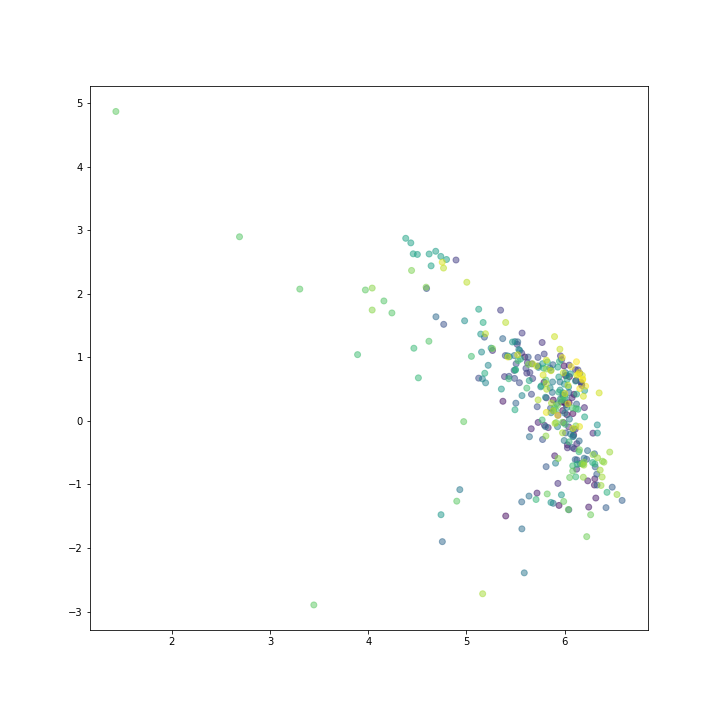
\includegraphics[scale=0.15]{newP1C3S3}
  \label{fig:test1}
\end{minipage}
\begin{minipage}{.5\textwidth}
  \captionof{figure}{Bach: Sinfonia No. 4}
  \centering
  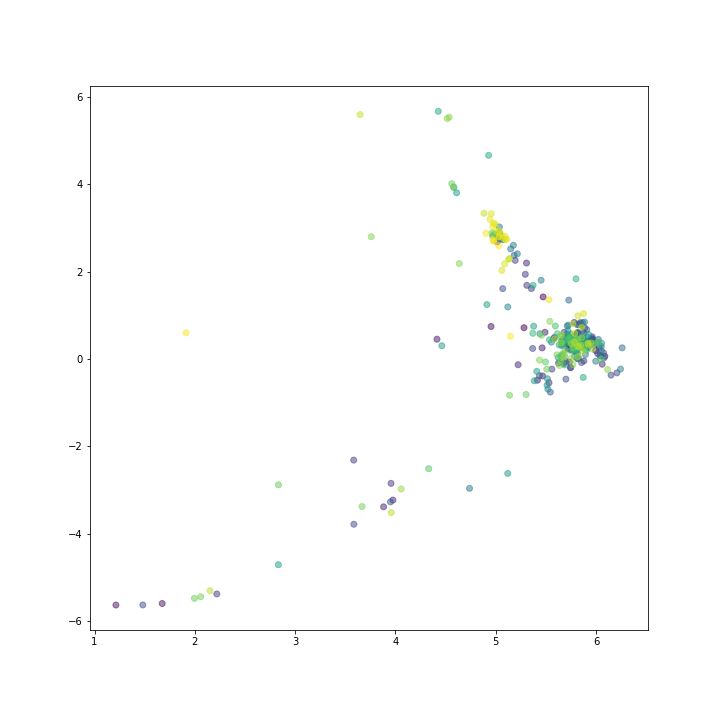
\includegraphics[scale=0.15]{newP1C5S4}
  \label{fig:test2}
\end{minipage}
\end{figure}

\begin{figure}[H]
\caption{3D Graph of P1C3S3 and P1C5S4}
\centering
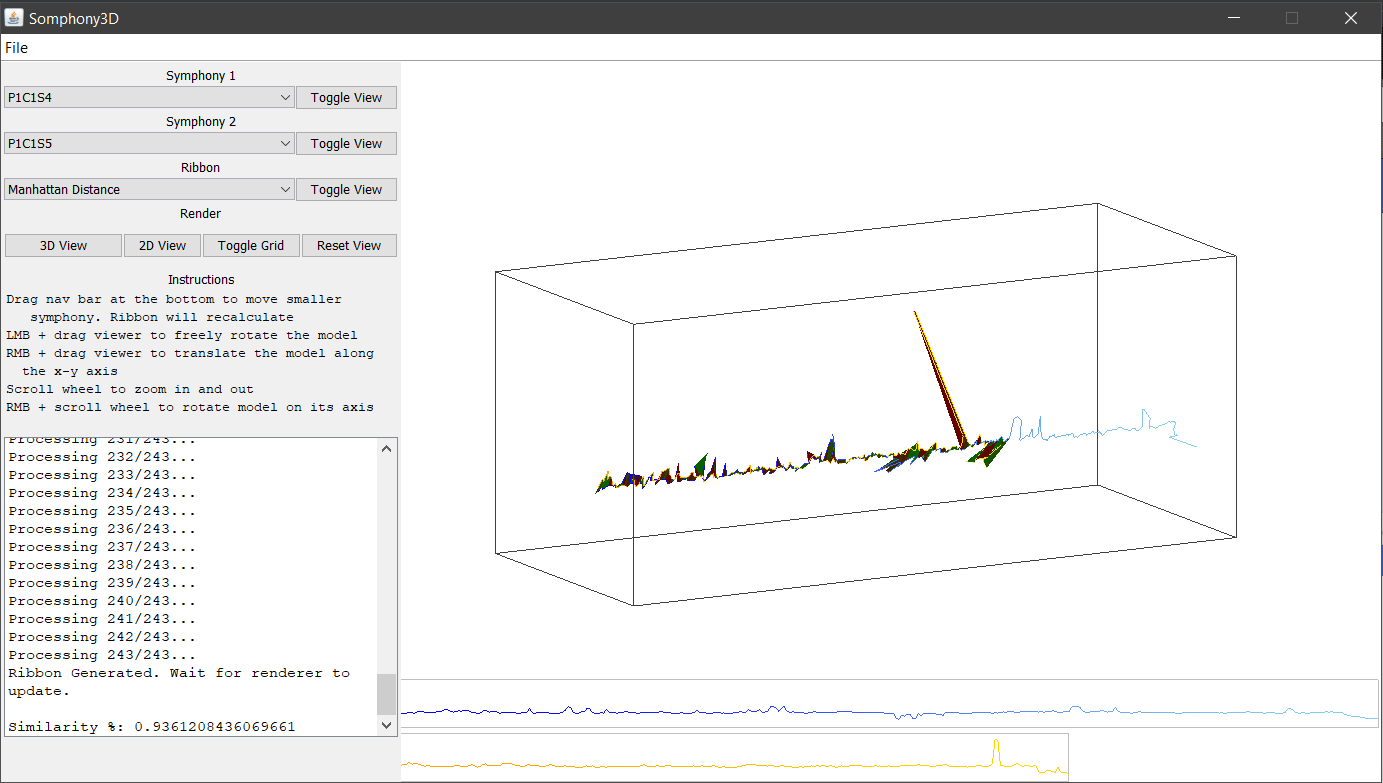
\includegraphics[scale=0.5]{comp1}
\end{figure}

\begin{longtable}{|l|l|l|}
\caption{Manhattan Distance Original Result}
\label{my-label}\\
\hline
Symphony A & Symphony B & Distance Mean \\ \hline
\endfirsthead
%
\endhead
%
P1C1S4 & P1C1S5 & 1.106247 \\ \hline
P1C3S3 & P1C5S4 & 1.888983 \\ \hline
P3C3S2 & P3C3S5 & 2.709862 \\ \hline
P1C1S5 & P1C5S3 & 2.71749 \\ \hline
P4C4S4 & P4C4S5 & 2.783062 \\ \hline
P3C2S1 & P3C3S1 & 2.885411 \\ \hline
P3C3S1 & P3C3S2 & 2.894063 \\ \hline
P1C3S3 & P1C5S3 & 3.051272 \\ \hline
P3C2S1 & P3C3S4 & 3.158728 \\ \hline
P1C1S4 & P1C5S3 & 3.180371 \\ \hline
P3C3S1 & P3C3S3 & 3.197033 \\ \hline
P3C3S2 & P3C3S3 & 3.213563 \\ \hline
P1C1S4 & P1C3S3 & 3.227913 \\ \hline
P3C3S1 & P3C3S4 & 3.303385 \\ \hline
P1C1S4 & P1C5S4 & 3.310048 \\ \hline
P1C1S1 & P3C5S3 & 3.356575 \\ \hline
P1C4S1 & P1C4S3 & 3.383625 \\ \hline
P3C2S1 & P3C3S2 & 3.384755 \\ \hline
P3C1S4 & P4C2S1A & 3.422252 \\ \hline
P1C1S1 & P1C3S2 & 3.433787 \\ \hline
P2C4S4A & P4C2S1A & 3.438686 \\ \hline
P1C1S1 & P3C1S1 & 3.472338 \\ \hline
P3C1S4 & P3C5S4 & 3.541771 \\ \hline
P3C4S5 & P4C2S1A & 3.548003 \\ \hline
P1C4S1 & P1C4S5 & 3.548142 \\ \hline
P1C5S1 & P4C3S5 & 3.583475 \\ \hline
P3C5S4 & P4C2S1A & 3.58519 \\ \hline
P3C2S1 & P3C3S3 & 3.594948 \\ \hline
P1C4S1 & P4C1S2A & 3.609206 \\ \hline
P2C4S4A & P3C1S4 & 3.637364 \\ \hline
P1C1S1 & P4C5S2 & 3.6608 \\ \hline
\end{longtable}

Table 5.4 below shows the result of Manhattan distance using the compressed data. Similarly, the longer of each pairwise symphonies were truncated when performing the Manhattan distances and the collective distances are thus averaged. Gabrieli\'s Canzon Duodecimi toni a 10 (P1C3S1) and Gabrieli\'s Canzon noni toni a 12 – Correggio (P1C3S3) were the top match with an average Manhattan distance of 1.69. Shown below in Figure 5.27 and 5.28 are the corresponding graphs of the pair. The pair now looks more similar than with the original data; however, there is still no strong similarity in the 2D graphs. This time, however, their cluster count based from Table 5.2 are no longer similar, with P1C3S1 having 93\% in E and only 6\% in B while P1C3S3 having 71\% in E and 28\% in B.

\begin{figure}[H]
\begin{minipage}{.5\textwidth}
  \captionof{figure}{Gabrieli: Canzon Duodecimi toni a 10}
  \centering
  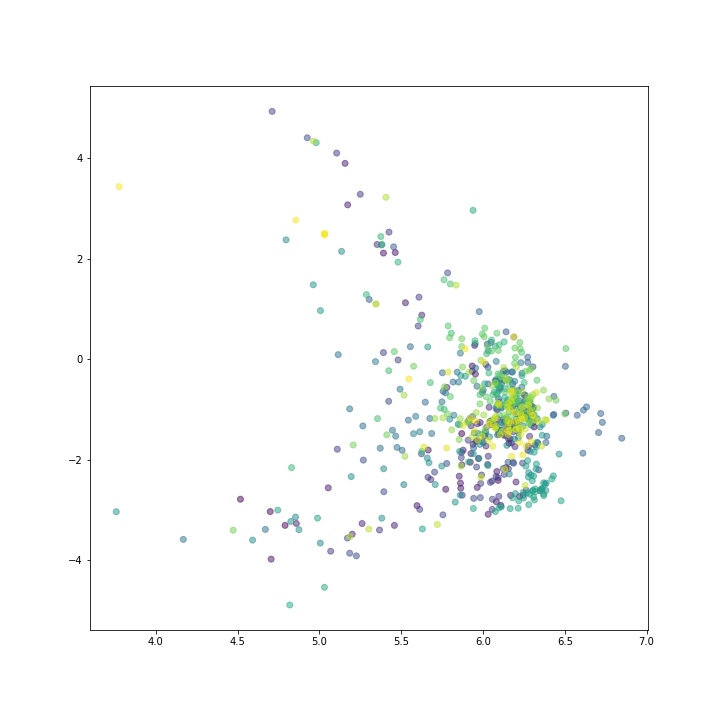
\includegraphics[scale=0.15]{newP1C3S1}
  \label{fig:test1}
\end{minipage}
\begin{minipage}{.5\textwidth}
  \captionof{figure}{Gabrieli: Canzon noni toni a 12 – Correggio}
  \centering
  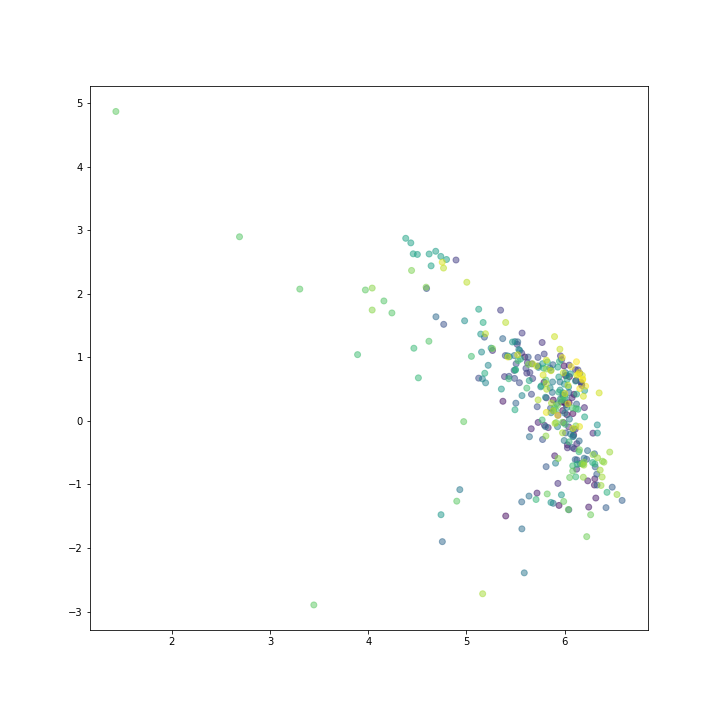
\includegraphics[scale=0.15]{newP1C3S3}
  \label{fig:test2}
\end{minipage}
\end{figure}

Again, the graphs shall be viewed in 3D to see if time played a role on the similarity of the pair. As seen in Figure 5.29 below, most of the ribbon are still colored green; however, the percentage similarity is now only 77\%.

\begin{figure}[H]
\caption{3D Graph of P1C3S1 and P1C3S3}
\centering
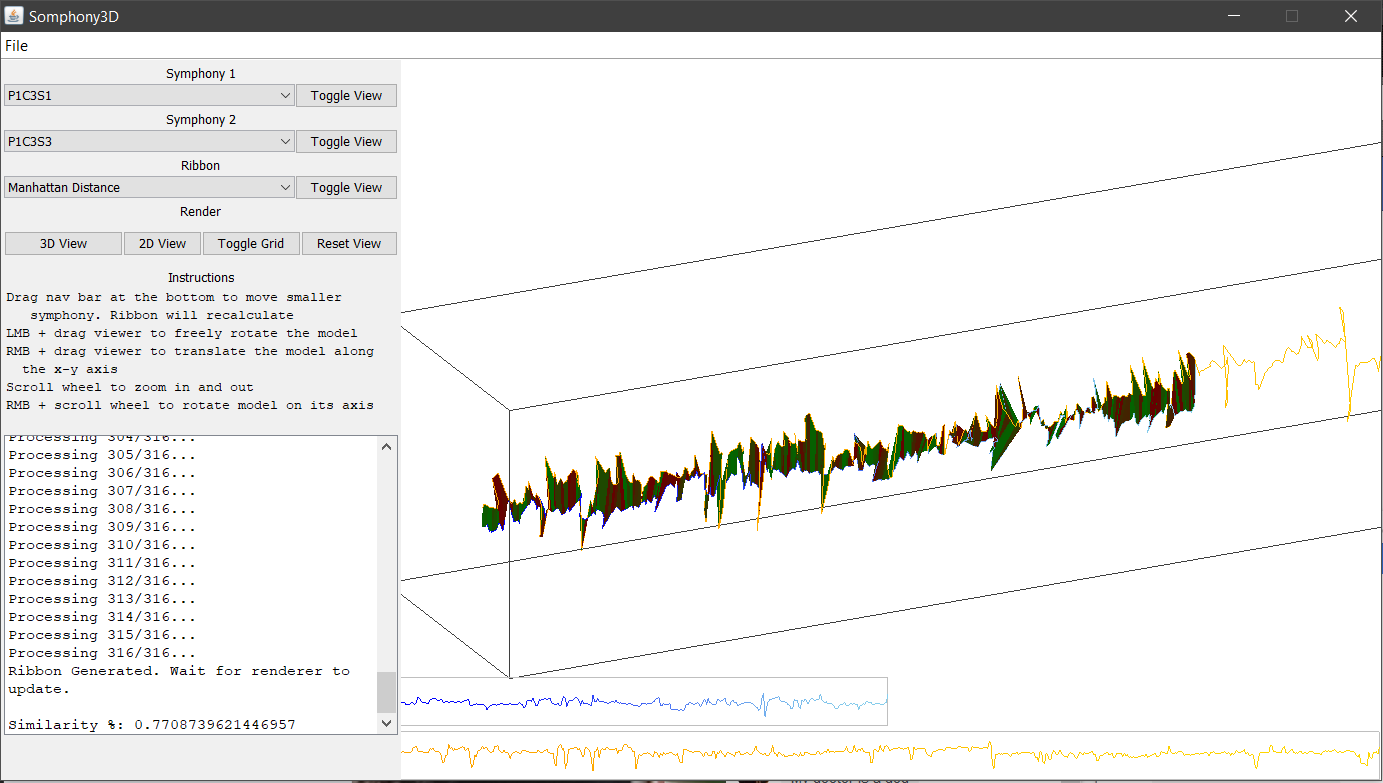
\includegraphics[scale=0.5]{comp2}
\end{figure}

\begin{longtable}{|l|l|l|}
\caption{Manhattan Distance Compressed Result}
\label{my-label}\\
\hline
Symphony A & Symphony B & Distance Mean \\ \hline
\endfirsthead
%
\endhead
%
P1C3S1 & P1C3S3 & 1.696353309 \\ \hline
P1C3S3 & P1C5S4 & 2.126664331 \\ \hline
P1C1S4 & P2C3S1A & 2.297832753 \\ \hline
P1C3S1 & P1C5S4 & 2.461786717 \\ \hline
P3C3S1 & P3C3S5 & 2.466141032 \\ \hline
P3C3S1 & P3C3S2 & 2.551953281 \\ \hline
P3C3S2 & P3C3S5 & 2.564866152 \\ \hline
P1C1S1 & P1C3S2 & 2.569937456 \\ \hline
P1C1S1 & P3C1S1 & 2.703949414 \\ \hline
P1C1S4 & P3C1S2 & 2.710989293 \\ \hline
P3C3S1 & P3C3S4 & 2.748674242 \\ \hline
P1C3S3 & P1C5S2 & 2.749400728 \\ \hline
P1C1S4 & P2C5S3A & 2.759343787 \\ \hline
P1C1S1 & P3C5S3 & 2.89002101 \\ \hline
P1C1S1 & P1C4S1 & 2.930982991 \\ \hline
P3C3S2 & P3C3S4 & 2.946366998 \\ \hline
P1C1S1 & P1C4S3 & 2.969399095 \\ \hline
P3C3S3 & P3C3S5 & 2.997141424 \\ \hline
P1C1S4 & P1C2S5 & 3.019357516 \\ \hline
P4C2S1A & P4C2S5 & 3.107856552 \\ \hline
P1C1S1 & P3C4S3 & 3.10991521 \\ \hline
P1C4S1 & P3C1S1 & 3.129107393 \\ \hline
P1C4S1 & P3C5S3 & 3.129297274 \\ \hline
P1C4S1 & P1C4S3 & 3.152097396 \\ \hline
P3C3S4 & P3C3S5 & 3.152275501 \\ \hline
P1C4S1 & P2C5S2A & 3.177974942 \\ \hline
P3C3S1 & P3C3S3 & 3.188811801 \\ \hline
P1C1S5 & P5C3S1A & 3.195726451 \\ \hline
P1C1S1 & P4C5S2 & 3.200008271 \\ \hline
P3C3S2 & P3C3S3 & 3.210794633 \\ \hline
\end{longtable}

Table 5.5 below shows the top results when longest common subsequence (LCS) is used with the original data using the cluster labels as strings as was discussed back in Chapter 4. Salieri\'s Sinfonia Veneziana in D major A (P2C5S4) and Rachmaninoff\'s Isle of the Dead (P5C2S2) is the top matching pair with a percent match of 56\%. This percentage was obtained by normalizing the resulting longest match between the two strings by dividing it with the length of the longer string between the pair. As shown in Figure 5.30 and Figure 5.31, both these symphonies indeed show a strong similarity with each other. This result may point to the direction that LCS is a good metric for comparing similarities between symphonies. Table 5.2 shows that both symphonies have evenly distributed points among the clusters; however, the distributions are not exactly near with P2C5S4 having 26\%, 26\%, 15\%, 33\%, and 1\% respectively, and P5C2S2 having 42\%, 11\%, 20\%, 24\%, and 3\%.

Figure 5.32 shows the 3D results of the two symphonies. The percentage similarity is now only 69\% with many parts of the ribbon now being red. This shows that while LCS provides good comparison with the 2D graph, when time is now incorporated, the result shows now that the percentage match isn\'t that high afterall.

\begin{figure}[H]
\begin{minipage}{.5\textwidth}
  \captionof{figure}{ Salieri: Sinfonia Veneziana in D major A}
  \centering
  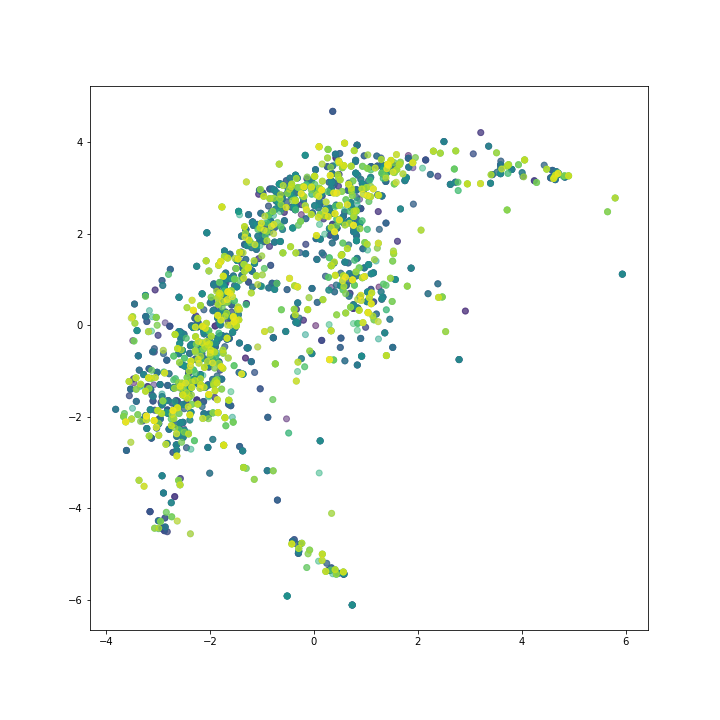
\includegraphics[scale=0.15]{newP2C5S4A}
  \label{fig:test1}
\end{minipage}
\begin{minipage}{.5\textwidth}
  \captionof{figure}{Rachmaninoff: Isle of the Dead}
  \centering
  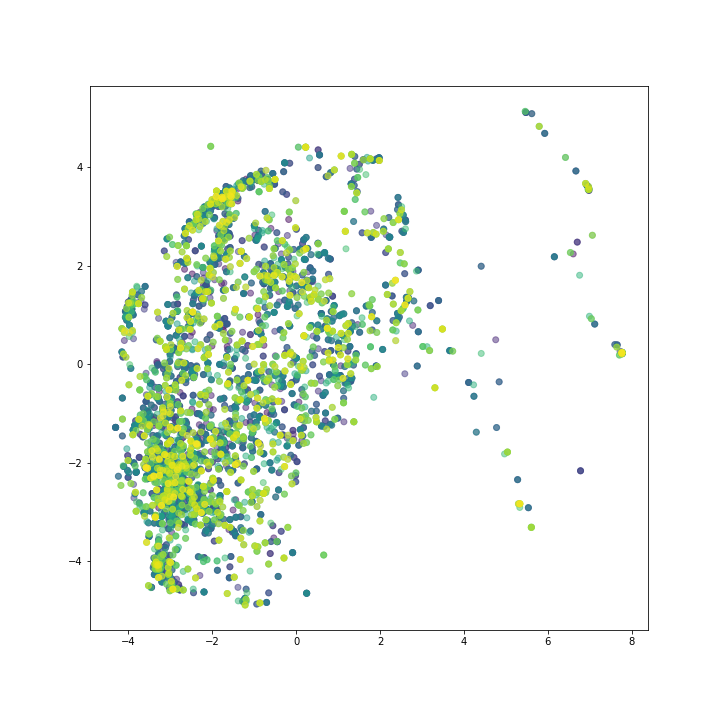
\includegraphics[scale=0.15]{newP5C2S2A}
  \label{fig:test2}
\end{minipage}
\end{figure}

\begin{figure}[H]
\caption{3D Graph of P2C5S4 and P5C2S2}
\centering
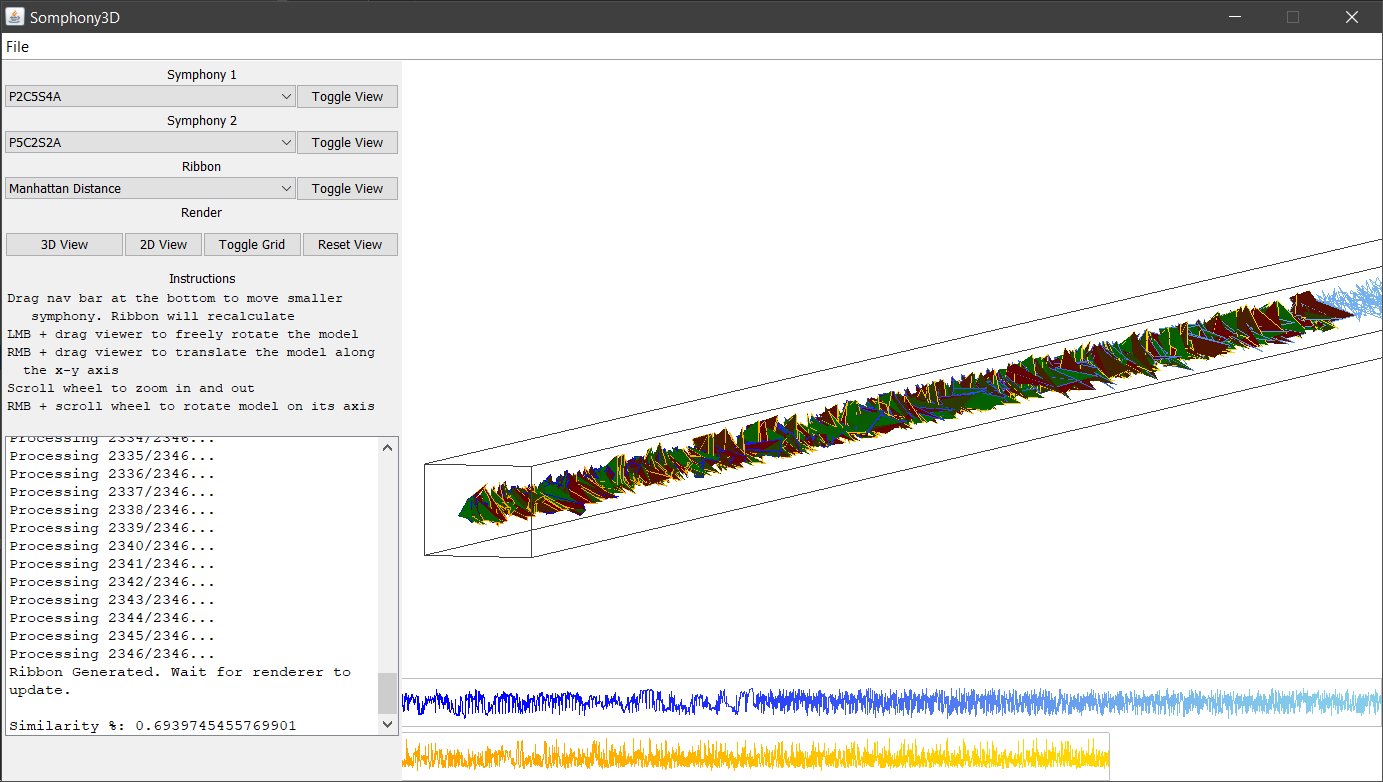
\includegraphics[scale=0.5]{comp3}
\end{figure}

\begin{longtable}{|l|l|l|}
\caption{LCS Original Result}
\label{my-label}\\
\hline
Symphony A & Symphony B & Percent Match \\ \hline
\endfirsthead
%
\endhead
%
P2C5S4A & P5C2S2A & 0.559178289 \\ \hline
P2C4S4A & P5C3S5A & 0.545797211 \\ \hline
P2C5S4A & P5C4S2A & 0.53618545 \\ \hline
P2C4S4A & P5C5S3 & 0.52977761 \\ \hline
P2C5S4A & P5C4S3A & 0.526950622 \\ \hline
P2C5S4A & P5C5S5A & 0.514134942 \\ \hline
P2C5S4A & P5C2S1A & 0.505277045 \\ \hline
P2C5S4A & P4C1S2A & 0.500565398 \\ \hline
P2C4S1A & P5C3S5A & 0.494911421 \\ \hline
P2C5S4A & P5C4S4A & 0.494534489 \\ \hline
P2C5S3A & P5C2S2A & 0.492272899 \\ \hline
P2C4S1A & P5C5S3 & 0.491519035 \\ \hline
P2C5S1A & P5C3S5A & 0.486807388 \\ \hline
P2C5S4A & P5C3S1A & 0.485865058 \\ \hline
P2C4S4A & P5C2S4A & 0.481341877 \\ \hline
P2C5S4A & P5C3S2A & 0.481341877 \\ \hline
P2C4S4A & P5C5S4 & 0.474934037 \\ \hline
P2C1S4 & P5C5S3 & 0.473614776 \\ \hline
P2C4S4A & P5C5S1A & 0.470976253 \\ \hline
P2C5S4A & P5C3S3A & 0.46701847 \\ \hline
P2C4S4A & P4C2S1A & 0.463626084 \\ \hline
P2C1S4 & P5C3S3A & 0.463437618 \\ \hline
P2C5S4A & P5C4S5A & 0.463437618 \\ \hline
P2C1S4 & P5C2S5A & 0.463060686 \\ \hline
P2C5S3A & P5C2S1A & 0.459102902 \\ \hline
P2C1S4 & P5C3S2A & 0.453071994 \\ \hline
P2C1S4 & P5C2S1A & 0.451752733 \\ \hline
P2C5S4A & P5C4S1A & 0.451187335 \\ \hline
P2C5S2A & P5C2S2A & 0.447983415 \\ \hline
P2C5S3A & P5C3S2A & 0.447229551 \\ \hline
\end{longtable}

Table 5.6 below shows the result of LCS performed on the compressed data. Viadana\'s Sinfonia la Bolognese (P2C5S4) and Rachmaninoff\'s Isle of the Dead (P5C2S2) are the top match, which is the same with the result of LCS performed on the original data. Having the same result, which also happens to be a very good result, since they are indeed similar-looking, means that LCS indeed may be a very good metric for comparison of symphonies using this particular methodology.

\begin{longtable}{|l|l|l|}
\caption{LCS  Compressed Result}
\label{my-label}\\
\hline
Symphony A & Symphony B & Percentage Match \\ \hline
\endfirsthead
%
\endhead
%
P2C5S4A & P5C2S2A & 42\% \\ \hline
P5C5S5A & P5C2S2A & 41\% \\ \hline
P5C4S3A & P5C5S5A & 41\% \\ \hline
P5C5S5A & P5C4S3A & 41\% \\ \hline
P5C2S1A & P5C2S2A & 41\% \\ \hline
P2C5S4A & P5C4S3A & 41\% \\ \hline
P5C4S2A & P5C5S5A & 40\% \\ \hline
P5C2S2A & P5C4S2A & 40\% \\ \hline
P5C2S2A & P5C4S3A & 40\% \\ \hline
P5C4S3A & P5C4S4A & 40\% \\ \hline
P2C5S4A & P5C4S2A & 40\% \\ \hline
P5C3S1A & P5C4S3A & 39\% \\ \hline
P5C2S2A & P5C3S2A & 39\% \\ \hline
P5C4S2A & P5C4S4A & 38\% \\ \hline
P5C4S3A & P5C5S1A & 38\% \\ \hline
P2C5S4A & P5C5S5A & 38\% \\ \hline
P5C3S2A & P5C4S3A & 37\% \\ \hline
P5C3S5A & P5C5S1A & 37\% \\ \hline
P2C5S4A & P5C2S1A & 37\% \\ \hline
P5C4S3A & P5C4S5A & 37\% \\ \hline
P5C1S4A & P5C1S5A & 37\% \\ \hline
P2C5S4A & P5C4S4A & 36\% \\ \hline
P5C3S5A & P5C5S3 & 36\% \\ \hline
P5C2S2A & P5C3S1A & 36\% \\ \hline
P5C4S4A & P5C5S5A & 36\% \\ \hline
P5C1S5A & P5C2S2A & 36\% \\ \hline
P5C2S2A & P5C4S4A & 36\% \\ \hline
P2C5S4A & P5C3S2A & 36\% \\ \hline
P2C5S4A & P5C3S1A & 35\% \\ \hline
P5C2S1A & P5C4S3A & 35\% \\ \hline
\end{longtable}

Table 5.7 below shows the result of Levenshtein distance using the original data. Given the trajectory of the symphony, which is represented by letters from A to E, the researchers compared all of the symphonies and normalized the results by dividing the distance with the length of the longer symphony. Bach\'s Brandenburg Concerto No.3 (P1C1S3) and Rubinstein\'s Symphony No.6 in A minor Op.111 (P3C5S5) had the least distance with only 0.13. Looking at their 2D graphs in Figure 5.33 and Figure 5.34, there is a slight similarity between the two in the positioning of the points; however, the visual output of the 2D graph does not show the closeness of the two symphonies. Looking at the 3D graph in Figure 5.35 though, it can be seen that 
the percentage similarity is 71\% which is quite low compared to that of Manhattan distance.

\begin{figure}[H]
\begin{minipage}{.5\textwidth}
  \captionof{figure}{Bach: Brandenburg Concerto No.3}
  \centering
  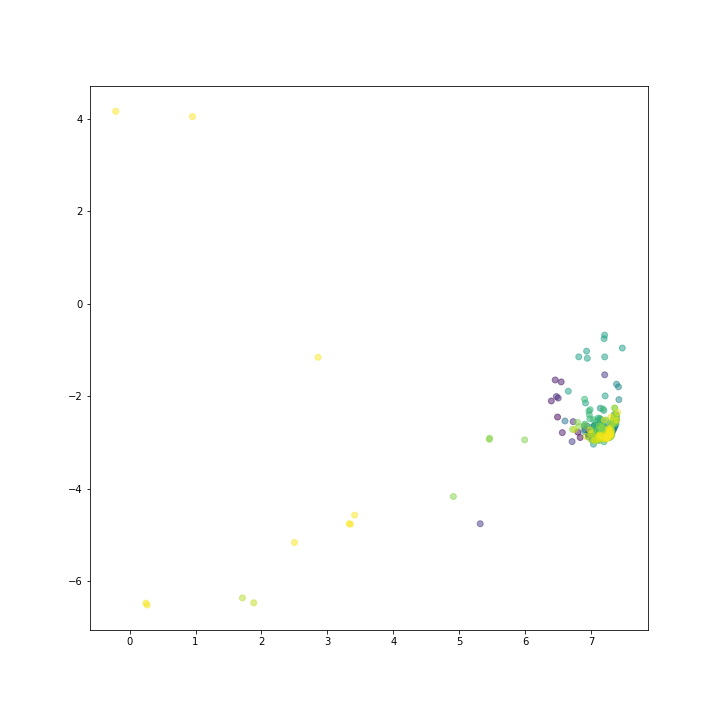
\includegraphics[scale=0.15]{newP1C1S3}
  \label{fig:test1}
\end{minipage}
\begin{minipage}{.5\textwidth}
  \captionof{figure}{Rubinstein: Symphony No.6 in A minor Op.111}
  \centering
  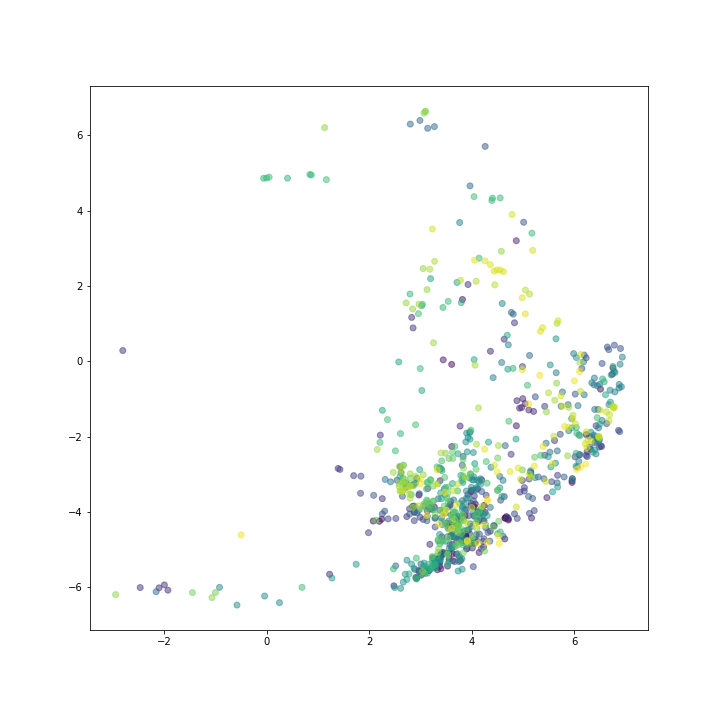
\includegraphics[scale=0.15]{newP3C5S5}
  \label{fig:test2}
\end{minipage}
\end{figure}

\begin{figure}[H]
\caption{3D Graph of P1C1S3 and P3C5S5}
\centering
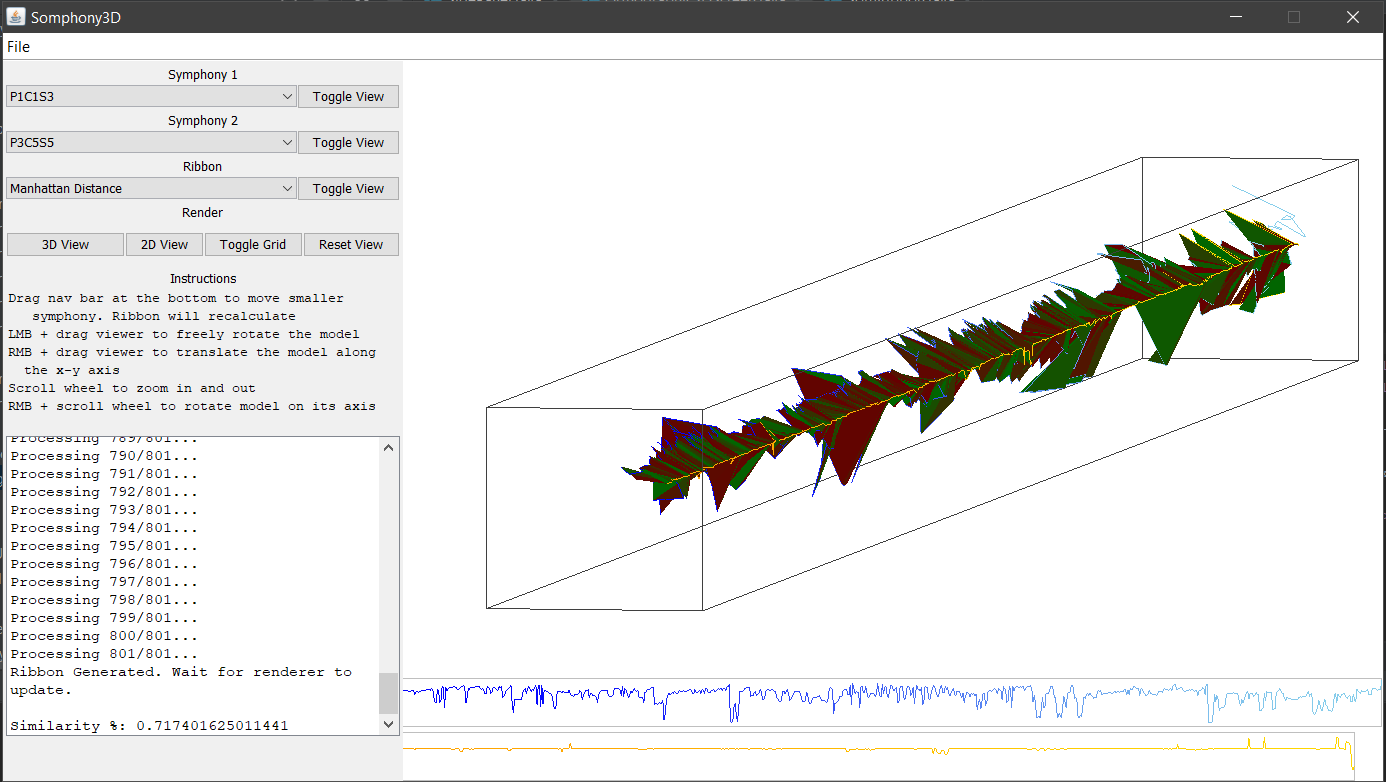
\includegraphics[scale=0.5]{comp5}
\end{figure}

\begin{longtable}{|l|l|l|}
\caption{Levenshtein Distance Original Result}
\label{my-label}\\
\hline
Symphony A & Symphony B & Distance \\ \hline
\endfirsthead
%
\endhead
%
P1C1S3 & P3C5S5 & 0.13 \\ \hline
P4C4S4 & P4C4S5 & 0.14 \\ \hline
P1C2S2 & P1C5S1 & 0.17 \\ \hline
P1C1S3 & P1C4S2 & 0.20 \\ \hline
P1C4S2 & P3C5S5 & 0.25 \\ \hline
P1C3S1 & P3C5S5 & 0.25 \\ \hline
P1C4S4 & P3C1S5 & 0.25 \\ \hline
P1C1S3 & P1C3S1 & 0.26 \\ \hline
P4C3S5 & P5C5S2 & 0.27 \\ \hline
P1C1S5 & P1C5S3 & 0.27 \\ \hline
P1C4S4 & P2C3S3 & 0.28 \\ \hline
P3C2S1 & P3C3S3 & 0.28 \\ \hline
P3C3S4 & P4C4S5 & 0.28 \\ \hline
P1C1S4 & P1C5S2 & 0.28 \\ \hline
P3C3S4 & P4C4S4 & 0.29 \\ \hline
P1C3S3 & P1C5S4 & 0.31 \\ \hline
P1C1S5 & P1C5S2 & 0.32 \\ \hline
P1C1S4 & P1C1S5 & 0.32 \\ \hline
P2C3S2 & P3C1S5 & 0.32 \\ \hline
P1C4S2 & P2C3S2 & 0.33 \\ \hline
P2C3S2 & P3C5S5 & 0.33 \\ \hline
P1C4S2 & P3C1S5 & 0.34 \\ \hline
P4C3S1 & P4C3S2 & 0.34 \\ \hline
P3C3S1 & P3C3S5 & 0.34 \\ \hline
P3C2S1 & P3C3S1 & 0.34 \\ \hline
P1C2S4 & P2C3S5 & 0.34 \\ \hline
P1C2S3 & P1C3S1 & 0.34 \\ \hline
P3C3S2 & P3C3S5 & 0.34 \\ \hline
P3C2S1 & P3C3S5 & 0.34 \\ \hline
P3C3S1 & P3C3S2 & 0.35 \\ \hline
\end{longtable}

Table 5.8 below shows the result of Levenshtein distance using the compressed data. The resulting distances are, again, normalized to prevent bias to symphony lengths. As shown in Figure 5.36 and Figure 5.37, the graphs do not share a large similarity, but they are somewhat located near the same coordinates. Figure 5.38 shows that there is a large similarity, however, between these two symphonies with a similarity percentage of 86\%.

\begin{figure}[H]
\begin{minipage}{.5\textwidth}
  \captionof{figure}{Gossec: Symphony in E-flat major Op.XII No.5}
  \centering
  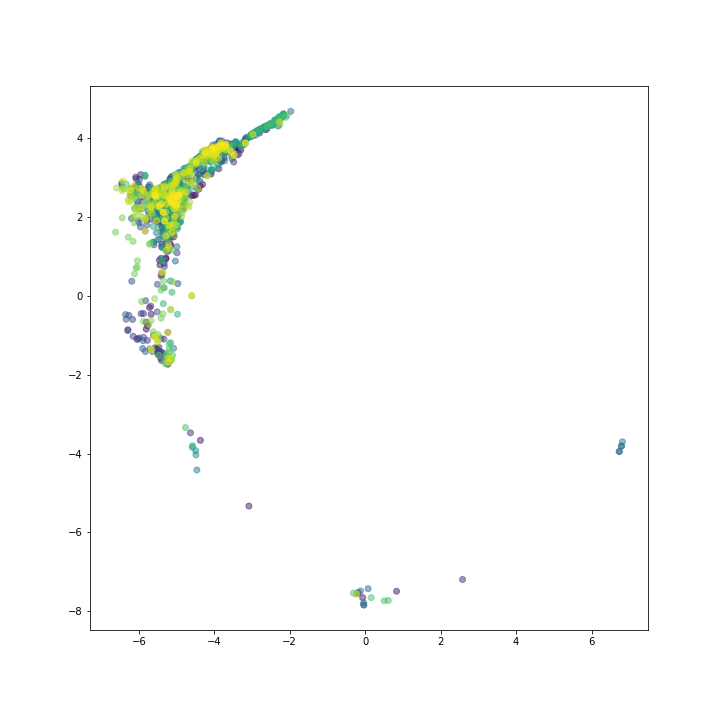
\includegraphics[scale=0.15]{newP3C3S2}
  \label{fig:test1}
\end{minipage}
\begin{minipage}{.5\textwidth}
  \captionof{figure}{Schubert: Symphony No.5 in B-flat major}
  \centering
  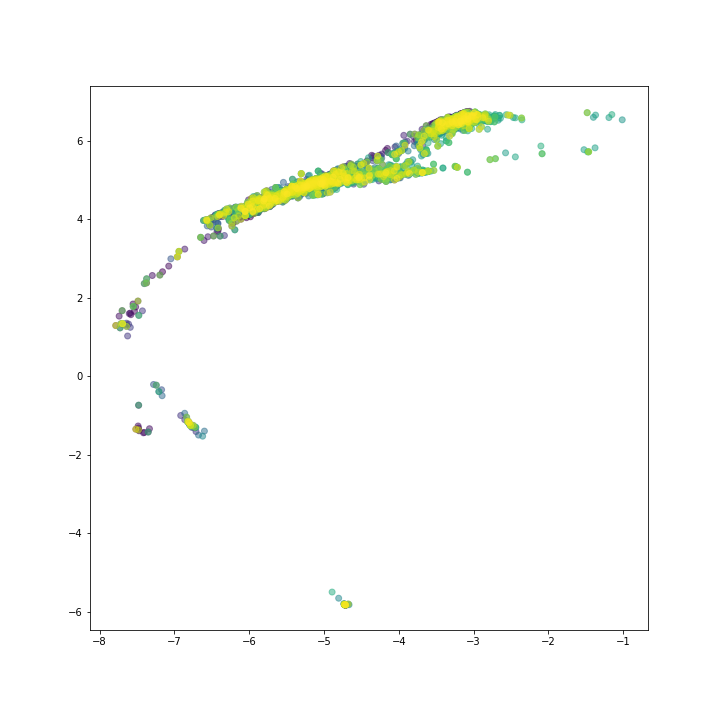
\includegraphics[scale=0.15]{newP4C3S3}
  \label{fig:test2}
\end{minipage}
\end{figure}

\begin{figure}[H]
\caption{3D Graph of P3C3S2 and P4C3S3}
\centering
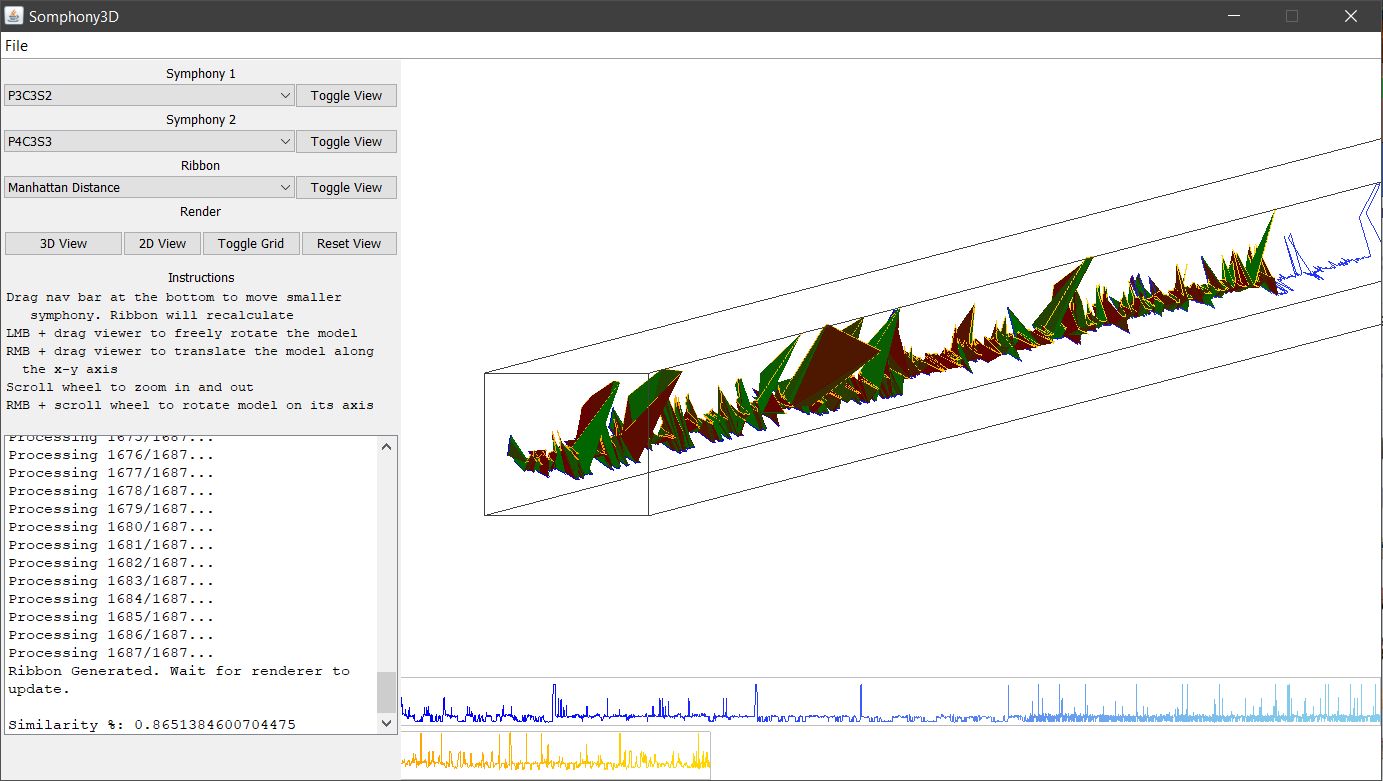
\includegraphics[scale=0.5]{comp6}
\end{figure}

\begin{longtable}{|l|l|l|}
\caption{Levenshtein Disance Result (Compressed)}
\label{my-label}\\
\hline
Symphony A & Symphony B & Distance \\ \hline
\endfirsthead
%
\endhead
%
P3C3S2 & P4C3S3 & 0.0067 \\ \hline
P1C1S3 & P1C1S5 & 0.0075 \\ \hline
P3C2S1 & P4C3S2 & 0.0096 \\ \hline
P1C1S3 & P1C1S4 & 0.0100 \\ \hline
P3C3S2 & P4C3S2 & 0.0111 \\ \hline
P4C3S2 & P4C3S3 & 0.0116 \\ \hline
P3C3S5 & P4C3S3 & 0.0118 \\ \hline
P1C3S1 & P1C5S4 & 0.0126 \\ \hline
P1C5S1 & P4C3S5 & 0.0126 \\ \hline
P1C3S3 & P4C3S5 & 0.0133 \\ \hline
P1C2S2 & P4C3S5 & 0.0136 \\ \hline
P1C1S3 & P1C3S4 & 0.0137 \\ \hline
P3C3S3 & P4C3S2 & 0.0148 \\ \hline
P1C1S5 & P1C3S4 & 0.0151 \\ \hline
P1C5S2 & P4C3S5 & 0.0161 \\ \hline
P3C5S5 & P4C3S5 & 0.0163 \\ \hline
P4C4S4 & P4C4S5 & 0.0166 \\ \hline
P3C1S2 & P4C3S5 & 0.0168 \\ \hline
P3C2S1 & P4C3S3 & 0.0170 \\ \hline
P1C4S1 & P4C3S5 & 0.0170 \\ \hline
P1C3S1 & P4C3S5 & 0.0180 \\ \hline
P4C3S5 & P4C4S5 & 0.0180 \\ \hline
P1C5S4 & P4C3S5 & 0.0183 \\ \hline
P1C2S3 & P4C3S5 & 0.0185 \\ \hline
P1C3S1 & P1C5S2 & 0.0188 \\ \hline
P1C2S4 & P4C3S5 & 0.0190 \\ \hline
P3C2S3 & P4C3S5 & 0.0193 \\ \hline
P3C3S3 & P4C4S4 & 0.0197 \\ \hline
P1C1S3 & P1C5S3 & 0.0200 \\ \hline
P3C2S2 & P4C3S5 & 0.0200 \\ \hline
\end{longtable}

In order to verify which metric was the best, we compare the top 30 most similar pairs of symphonies generated by each metric and find out which two metrics had the most matches. Based on Table 5.19 below, Manhattan distance got the top match between its original and compressed version, followed by LCS between its original and compressed version again. The first match between two completely different metric is Levenshtein distance with Manhattan distance, both using the original dataset, with a match of 6/30.

Most of the entries in the last few spots are dominated by the compressed dataset, which means that using compressed data for metric comparison has a large variance among each other in terms of the results produced by each metric.

\begin{longtable}{|l|l|l|}
\caption{Metric Evaluation for Pairwise Comparison of Symphonies}
\label{my-label}\\
\hline
Metric 1 & Metric 2 & Number of Matches \\ \hline
\endfirsthead
%
\endhead
%
MD Original & MD Compressed & 10 \\ \hline
LCS Compressed & LCS Original & 9 \\ \hline
LD Original & MD Original & 6 \\ \hline
LD Compressed & LD Original & 6 \\ \hline
LD Compressed & MD Original & 4 \\ \hline
MD Original & LCS Original & 2 \\ \hline
LD Original & MD Compressed & 2 \\ \hline
LCS Compressed & MD Original & 1 \\ \hline
LCS Compressed & LD Original & 1 \\ \hline
LCS Compressed & LD Compressed & 1 \\ \hline
LD Original & LCS Original & 1 \\ \hline
LD Transitions & MD Compressed & 1 \\ \hline
LD Transitions & LCS Original & 1 \\ \hline
LCS Compressed & MD Compressed & 0 \\ \hline
MD Compressed & LCS Original & 0 \\ \hline
\end{longtable}

\subsection{Composer Evaluation}

In order to evaluate which composers had the most similar compositions, we take the average of the distances per symphony made by each composer using pairwise comparisons of his compositions only. Table 5.10 shows the average number of edits per composer, under each era. The distances were also normalized prior to averaging by dividing the results by the length of the longer trajectory string. Figure 5.39 shows Antheil's graph. Each color, again, represents a particular symphony, blue for symphony 1, green for symphony 2, red for symphony 3, purple for symphony 4, and yellow for symphony 5. Figure 5.40 shows the individual symphonies of Antheil respectively. In Table 5.11, which shows Antheil\'s symphonies\' distances with one another in a correlation matrix, S2 and S3 had the least distance, which means they are the most similar according to Levenshtein distance. Also, the structure of S2 to S5 are very similar with each other visually which correlates to the finding that Antheil as a composer is deemed by Levenshtein distance as the composer with the most similar symphonies.

\begin{figure}[H]
\caption{Antheil Graph}
\centering
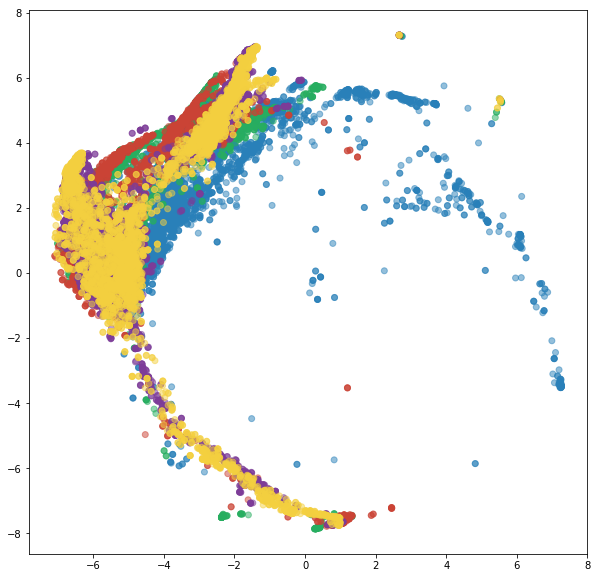
\includegraphics[scale=0.5]{P5C1}
\end{figure}

\begin{figure}[H]
\caption{Individual Symphony Graphs by Antheil}
\centering
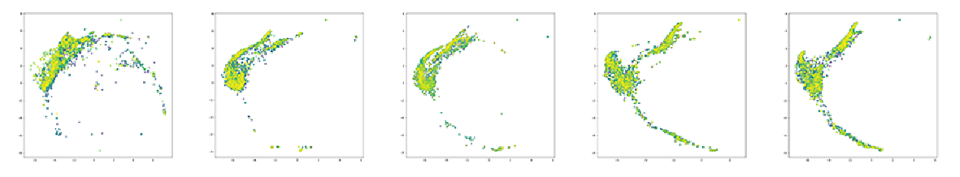
\includegraphics[scale=0.5]{antheil_symphonies}
\end{figure}

\begin{longtable}{|l|l|l|}
\caption{Average Normalized Levenshtein Distance per Composer}
\label{my-label}\\
\hline
Era & Composer & Percentage Similarity \\ \hline
\endfirsthead
%
\endhead
%
Baroque & Bach & 85\% \\ \hline
 & Boyce & 74\% \\ \hline
 & Gabrieli & 86\% \\ \hline
 & Sammartini & 78\% \\ \hline
 & Viadana & 74\% \\ \hline
Classical & Boccherini & 44\% \\ \hline
 & Gluck & 68\% \\ \hline
 & Haydn & 54\% \\ \hline
 & Mozart & 57\% \\ \hline
 & Salieri & 63\% \\ \hline
19th Century & Beethoven & 69\% \\ \hline
 & Clementi & 72\% \\ \hline
 & Gossec & 44\% \\ \hline
 & Kalliwoda & 64\% \\ \hline
 & Rubinstein & 72\% \\ \hline
Romantic & Dvorak & 71\% \\ \hline
 & Mendelssohn & 70\% \\ \hline
 & Schubert & 71\% \\ \hline
 & Schumann & 76\% \\ \hline
 & Tchaikovsky & 70\% \\ \hline
20th Century & Antheil & 44\% \\ \hline
 & Rachmaninoff & 66\% \\ \hline
 & Rubbra & 61\% \\ \hline
 & Shostakovich & 57\% \\ \hline
 & Stravinsky & 65\% \\ \hline
\end{longtable}

\begin{longtable}{|l|l|l|l|l|l|}
\caption{Antheil Matrix of Symphony Comparisons}
\label{my-label}\\
\hline
P5C1 & S1 & S2 & S3 & S4 & S5 \\ \hline
\endfirsthead
%
\endhead
%
S1 &  & 2853 & 2701 & 2847 & 2774 \\ \hline
S2 & 2853 &  & 2139 & 1857 & 2223 \\ \hline
S3 & 2701 & 2139 &  & 2329 & 2571 \\ \hline
S4 & 2847 & 1857 & 2329 &  & 2180 \\ \hline
S5 & 2774 & 2223 & 2571 & 2180 &  \\ \hline
\end{longtable}

The compressed trajectory strings also underwent normalized Levenshtein distance and the results are shown in Table 5.12. Antheil (P5C1) is shown to have the smallest average Levenshtein distance and as was shown in the graphs for Antheil, most of Antheil\'s symphonies really look alike.

\begin{longtable}{|l|l|l|}
\caption{Average Normalized Levenshtein Distance (Compressed) per Composer}
\label{my-label}\\
\hline
Era & Composer & Percentage Similarity \\ \hline
\endfirsthead
%
\endhead
%
Baroque & Bach & 87\% \\ \hline
 & Boyce & 70\% \\ \hline
 & Gabrieli & 81\% \\ \hline
 & Sammartini & 64\% \\ \hline
 & Viadana & 56\% \\ \hline
Classical & Boccherini & 58\% \\ \hline
 & Gluck & 64\% \\ \hline
 & Haydn & 38\% \\ \hline
 & Mozart & 49\% \\ \hline
 & Salieri & 57\% \\ \hline
19th Century & Beethoven & 62\% \\ \hline
 & Clementi & 69\% \\ \hline
 & Gossec & 58\% \\ \hline
 & Kalliwoda & 54\% \\ \hline
 & Rubinstein & 68\% \\ \hline
Romantic & Dvorak & 59\% \\ \hline
 & Mendelssohn & 54\% \\ \hline
 & Schubert & 63\% \\ \hline
 & Schumann & 72\% \\ \hline
 & Tchaikovsky & 58\% \\ \hline
20th Century & Antheil & 32\% \\ \hline
 & Rachmaninoff & 62\% \\ \hline
 & Rubbra & 53\% \\ \hline
 & Shostakovich & 49\% \\ \hline
 & Stravinsky & 54\% \\ \hline
\end{longtable}

Similarly, the result from Manhattan distance was tabulated to show the average distances of each composer per era as seen in Table 5.13. The result shows that Gossec of 19th Century  (P3C3) had the smallest distance value of 3.84 while Beethoven of 19th Century (P3C1) had the largest. This means that Gossec had symphonies that are very close with each other while Schubert had symphonies that are more dissimilar. Based from Table 5.14, S2 and S5 are the most similar among Gossec\'s symphonies. In the visual plots in Figure 5.41 and Figure 5.42 however, they look less alike than with S2 and S3 which appear to be more similar.

\begin{figure}[H]
\caption{Gossec Graph}
\centering
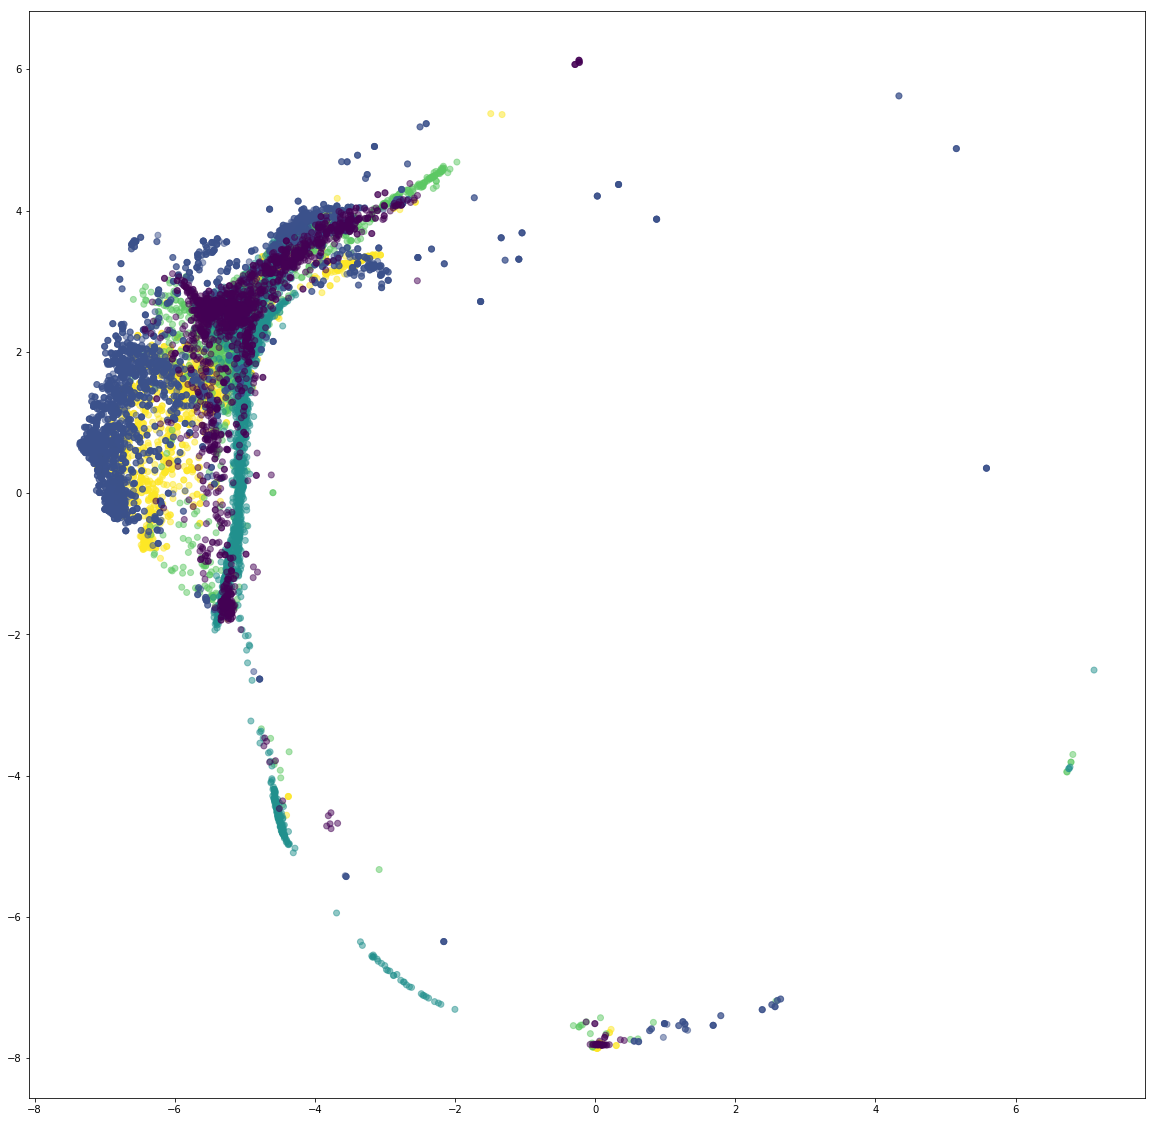
\includegraphics[scale=0.5]{P3C3}
\end{figure}

\begin{figure}[H]
\caption{Individual Symphony Graphs by Gossec}
\centering
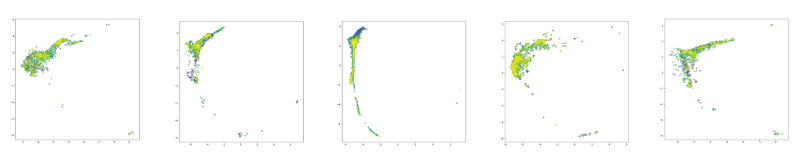
\includegraphics[scale=0.5]{gossec_symphonies}
\end{figure}

\begin{longtable}{|l|l|l|}
\caption{Average Manhattan Distance per Composer (Original)}
\label{my-label}\\
\hline
Era & Composer & Percentage Similarity \\ \hline
\endfirsthead
%
\endhead
%
Baroque & Bach & 7.14 \\ \hline
 & Boyce & 5.18 \\ \hline
 & Gabrieli & 6.05 \\ \hline
 & Sammartini & 6.59 \\ \hline
 & Viadana & 5.61 \\ \hline
Classical & Boccherini & 8.30 \\ \hline
 & Gluck & 5.33 \\ \hline
 & Haydn & 9.42 \\ \hline
 & Mozart & 6.27 \\ \hline
 & Salieri & 6.38 \\ \hline
19th Century & Beethoven & 10.45 \\ \hline
 & Clementi & 6.68 \\ \hline
 & Gossec & 3.84 \\ \hline
 & Kalliwoda & 9.59 \\ \hline
 & Rubinstein & 5.81 \\ \hline
Romantic & Dvorak & 6.89 \\ \hline
 & Mendelssohn & 5.36 \\ \hline
 & Schubert & 5.23 \\ \hline
 & Schumann & 8.01 \\ \hline
 & Tchaikovsky & 6.88 \\ \hline
20th Century & Antheil & 8.11 \\ \hline
 & Rachmaninoff & 5.78 \\ \hline
 & Rubbra & 5.82 \\ \hline
 & Shostakovich & 6.02 \\ \hline
 & Stravinsky & 8.53 \\ \hline
\end{longtable}

\begin{longtable}{|l|l|l|l|l|l|}
\caption{Gossec Matrix of Symphony Comparisons}
\label{my-label}\\
\hline
P3C3 & S1 & S2 & S3 & S4 & S5 \\ \hline
\endfirsthead
%
\endhead
%
S1 &  & 2.894063 & 3.197033 & 3.303385 & 4.294225 \\ \hline
S2 & 2.894063 &  & 3.213563 & 3.745208 & 2.709862 \\ \hline
S3 & 3.197033 & 3.213563 &  & 3.874635 & 4.016775 \\ \hline
S4 & 3.303385 & 3.745208 & 3.874635 &  & 7.194489 \\ \hline
S5 & 4.294225 & 2.709862 & 4.016775 & 7.194489 &  \\ \hline
\end{longtable}

Using Manhattan distance on the compressed data, the result can be seen in Table 5.15 and similarly, Gossec of 19th Century (P3C3) had the smallest distance of 2.98 while Beethoven still had the largest with 9.36. These results show that both the original data and the compressed data showed consistent results with both Manhattan distance and Levenshtein distance.

\begin{longtable}{|l|l|l|}
\caption{Average Manhattan Distance per Composer (Compressed)}
\label{my-label}\\
\hline
Era & Composer & Percentage Similarity \\ \hline
\endfirsthead
%
\endhead
%
Baroque & Bach & 5.81 \\ \hline
 & Boyce & 4.18 \\ \hline
 & Gabrieli & 5.01 \\ \hline
 & Sammartini & 5.61 \\ \hline
 & Viadana & 5.08 \\ \hline
Classical & Boccherini & 6.96 \\ \hline
 & Gluck & 4.76 \\ \hline
 & Haydn & 8.55 \\ \hline
 & Mozart & 4.60 \\ \hline
 & Salieri & 6.18 \\ \hline
19th Century & Beethoven & 9.36 \\ \hline
 & Clementi & 5.58 \\ \hline
 & Gossec & 2.98 \\ \hline
 & Kalliwoda & 8.62 \\ \hline
 & Rubinstein & 5.29 \\ \hline
Romantic & Dvorak & 6.32 \\ \hline
 & Mendelssohn & 4.93 \\ \hline
 & Schubert & 4.39 \\ \hline
 & Schumann & 7.89 \\ \hline
 & Tchaikovsky & 6.28 \\ \hline
20th Century & Antheil & 6.79 \\ \hline
 & Rachmaninoff & 5.40 \\ \hline
 & Rubbra & 5.50 \\ \hline
 & Shostakovich & 5.29 \\ \hline
 & Stravinsky & 7.67 \\ \hline
\end{longtable}